\documentclass[11pt]{article}
\usepackage{mystyle}

\title{Notes on \uct data resolution}
\author{Scott Trinkle}
\date{Last edited: \today}

\newsavebox{\largestimage}

\begin{document}

\maketitle

\section{Introduction}
In a recent group meeting, we discussed the idea of choosing the resolution of
the acquired \uct data to optimize the calculation of ODFs and segmentation of
white matter. The aim of these notes is to characterize the sensitivity of the
\uct ODFs to the resolution of the data. My hypothesis is that while acquiring
the data at a lower resolution will increase the accuracy and ease the
computational burden of segmenting white matter tracts, this will be at the
expense of ODF accuracy.

\section{Methods}
\subsection{Downscaling and ODF construction}
The same set of 225 ROI was used as in the
\href{https://github.com/scott-trinkle/uCTdMRI/blob/master/notes/2018-09-17-bit-depth/report/bit_depth_report.pdf}{previous
  notes} detailing the effect of bit depth and rescaling. For this study, the
original 32-bit data was used with no rescaling.

The native voxel size of the data is 1.2 \um. Each ROI was downsampled to four
smaller voxel sizes: 2.4~$\upmu$m~(2x), 3.6~\um~(3x), 4.8~\um~(4x), and
6.0~\um~(5x), using cubic spline interpolation. Structure tensor ODFs were then
calculated from all five scales for each ROI.  The optimized guassian filter
widths used in the structure tensor pipeline ($\sigma_d$ and $\sigma_n$,
optimized in
\href{https://github.com/scott-trinkle/uCTdMRI/tree/master/notes/2018-05-22-tuning-parameters/report}{previous
  notes}) were appropriately scaled to correspond to the same physical distance
at each resolution. Orientation estimates were not thresholded by FA value or
intensity before binning over 6500 uniform points on the sphere and expanding
onto even, real spherical harmonics, with $L_{max}=20$.

\subsection{Comparison metrics}
As in the
\href{https://github.com/scott-trinkle/uCTdMRI/blob/master/notes/2018-09-17-bit-depth/report/bit_depth_report.pdf}{bit
  depth notes}, ODFs calculated at different scales were compared using the ACC,
JSD, and RMSE of spherical harmonic coefficients. Additionally, the difference
in generalized fractional anisotropy was computed, defined as
\begin{align}
  \Delta\text{GFA} = \text{GFA}_{ds} - \text{GFA}_0,
\end{align}
where GFA$_{ds}$ is the GFA of the ODF calculated with downsampled data, and GFA$_0$ is the
GFA of the ODF calculated with the original data.

\section{Results}
Figure~\ref{fig:trends} shows the overall trends of the various comparison
metrics as a function of downsampling factor. All comparisons were done between
the original 1.2~\um~data and the downsampled data at various scales. The points
correspond to the mean comparison metric values for all 225 ROI at each
downsampling factor, and the error bars correspond to the standard deviations.

\begin{figure}[h]
  \centering
  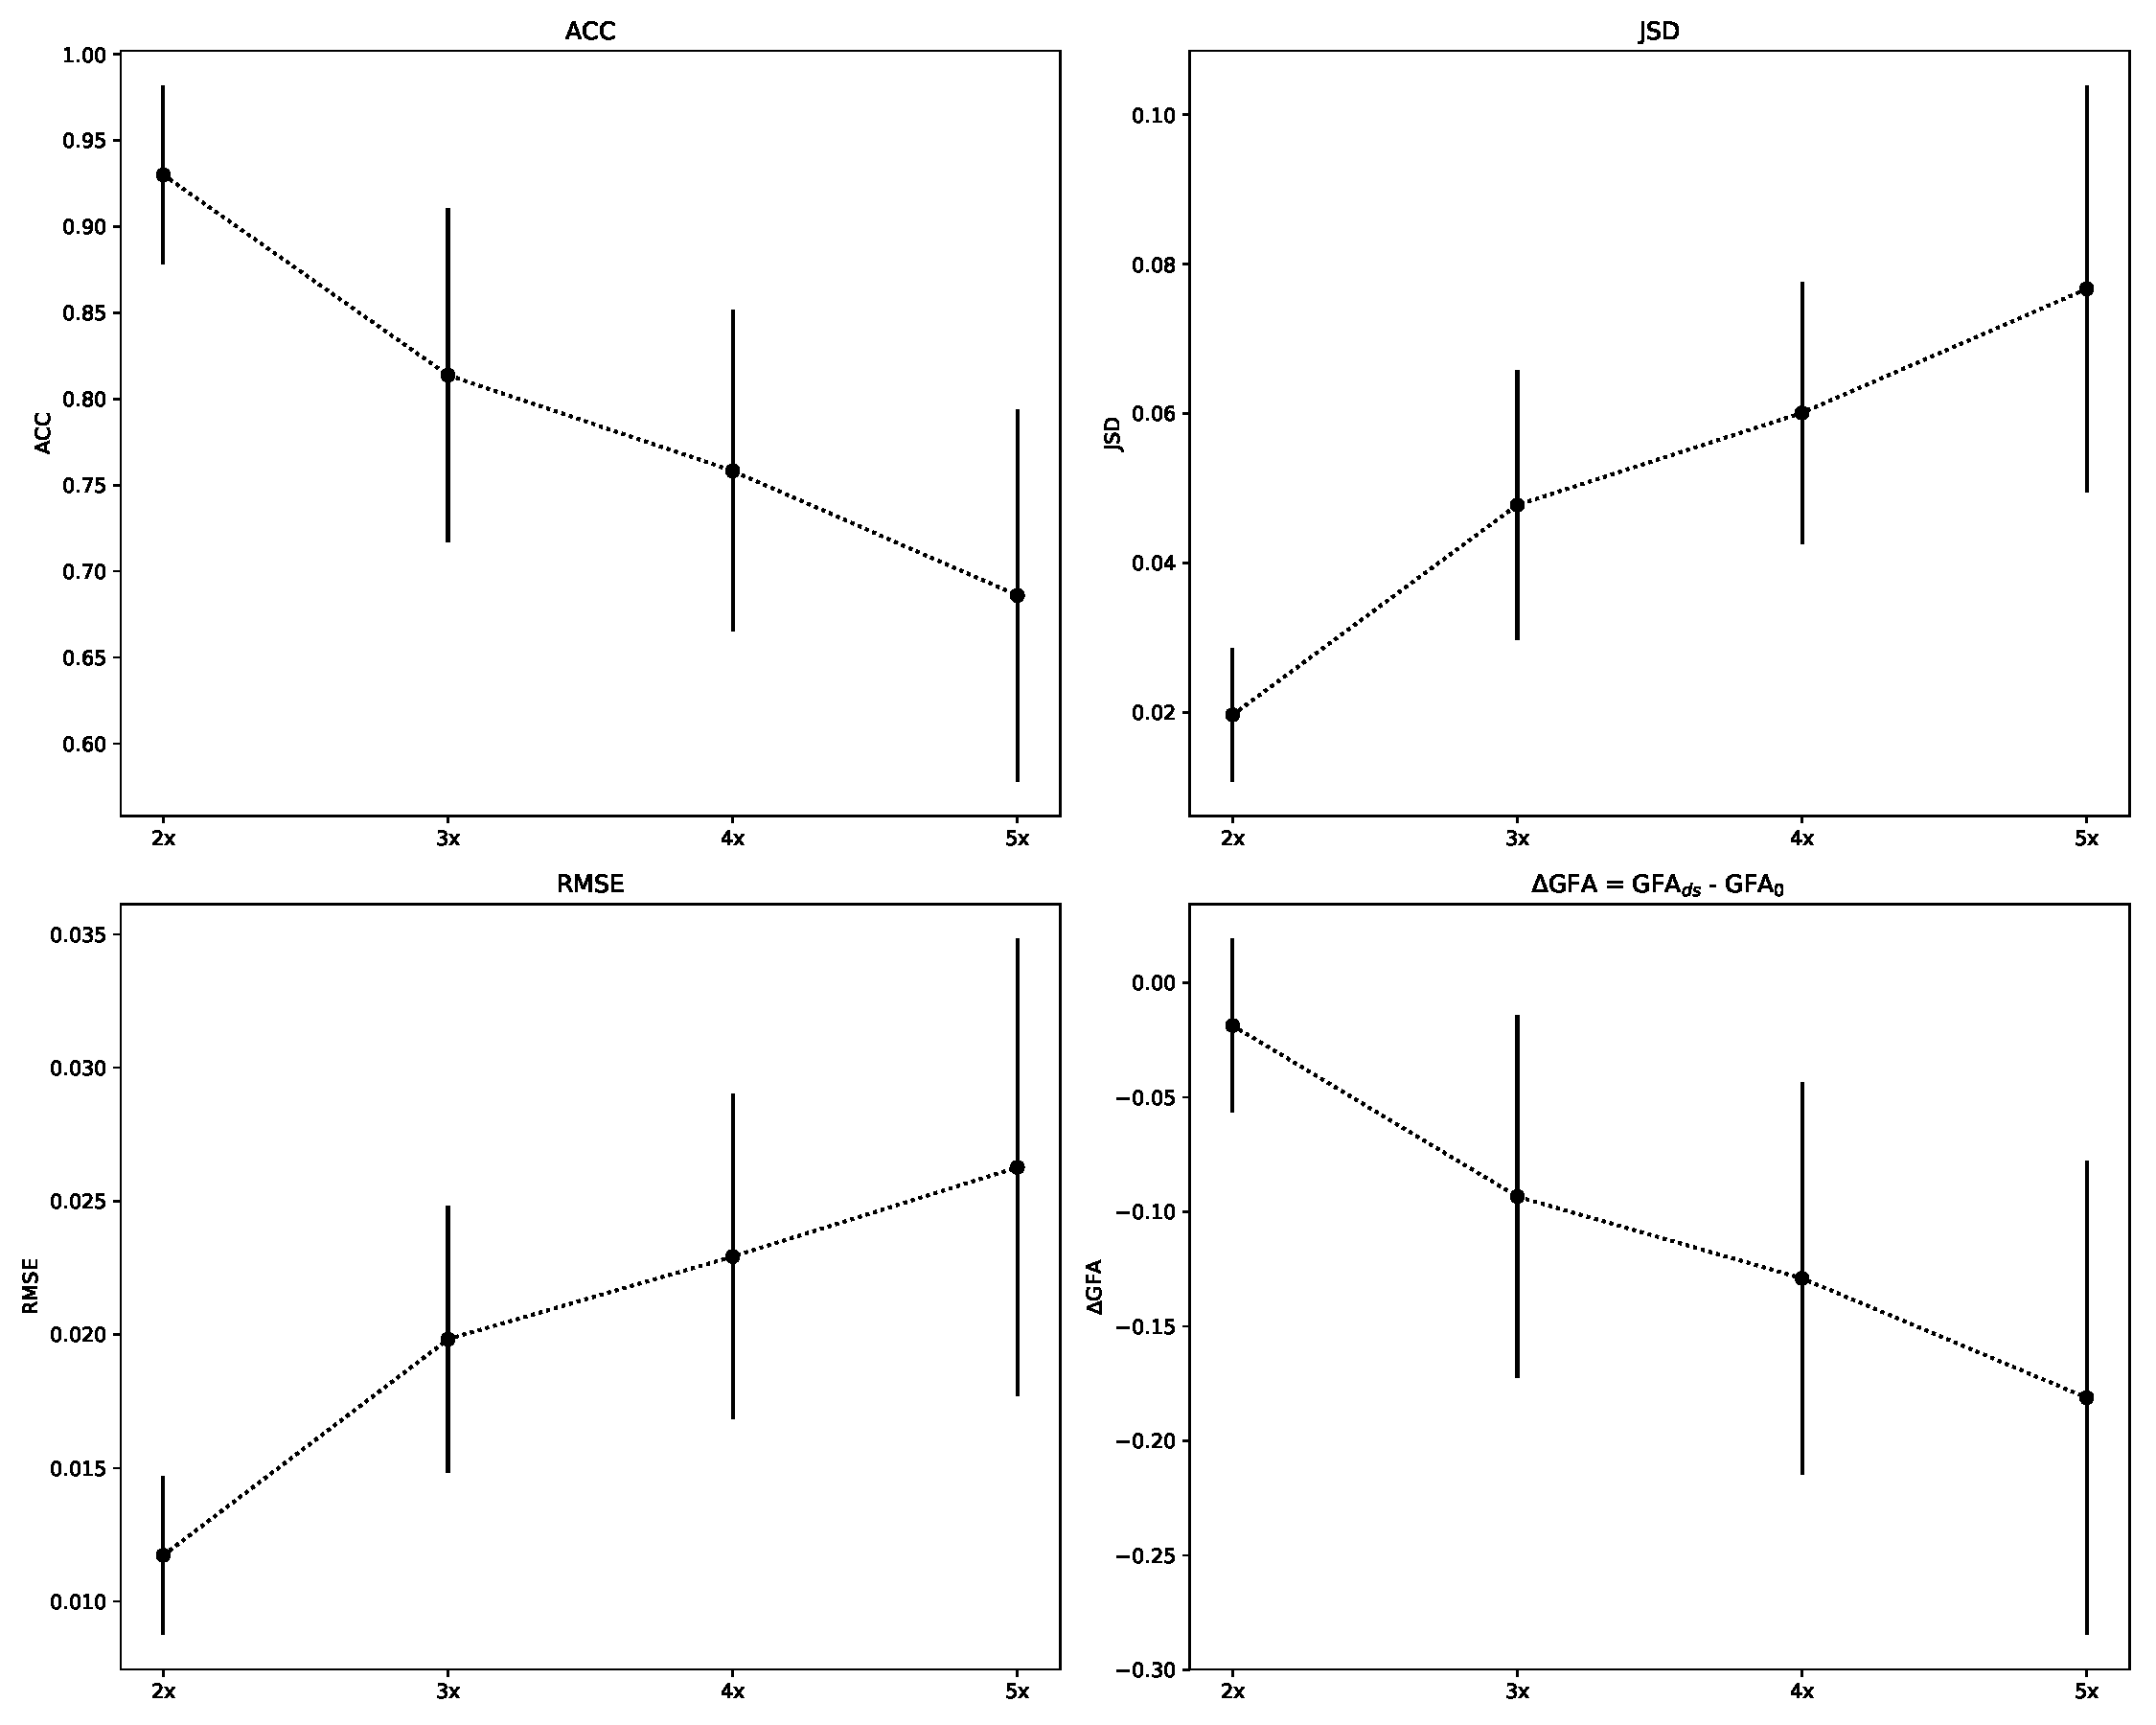
\includegraphics[width=\linewidth]{../plots/per_ds_factor}
  \caption{Comparison metric trends as a function of downsampling factor.}
  \label{fig:trends}
\end{figure}

As expected, the comparisons become worse --- i.e., the ODFs deviate more from
the full-resolution ``ground truth'' --- as the downsampling factor is
increased. Full distributions of these comparison metrics are appended to
these notes. 

Important to note is that the $\Delta$GFA tends to become more negative with
more downsampling. This indicates that the ODFs become increasingly isotropic
as we dicard more high-frequency content. Capturing anisotropic peaks in the 
ODFs is a fundamental task for all diffusion MRI reconstructions and forms
the basis of all tractography algorithms.

Figure~\ref{fig:odfs} gives a comparison of 1x and 2x ODFs for relatively
high values of ACC. Though the shapes are generally similar, it is clear
that there are discrepancies in the number and location of peaks. Even
for the ACC=0.95 case, the primary peaks are \textapprox 8$^\circ$ apart. 

\begin{center}
  \begin{longtable}{M{0.15\textwidth} M{0.3\textwidth} M{0.3\textwidth}}
    ACC & 1x ODF & 2x ODF\\
    0.85 & \im{0.3}{\odfpath{1x}{196}} & \im{0.3}{\odfpath{2x}{196}}\\
    0.90 & \im{0.3}{\odfpath{1x}{197}} & \im{0.3}{\odfpath{2x}{197}}\\
    0.95 & \im{0.3}{\odfpath{1x}{205}} & \im{0.3}{\odfpath{2x}{205}}\\
  \end{longtable}
  \captionsetup{width=0.9\textwidth}
  \captionof{figure}{Sample ODFs with ACC}   
  \label{fig:odfs}
\end{center}

\section{Conclusion}
These results seem to indicate that much of the oriented structure in the
\uct data is found in the high frequency content --- that acquiring the
data at a lower resolution will compromise the accuracy of the ODF.

A major issue that this potential strategy was brought up to address is the
significant computational challenge of segmenting individual axon bundles
throughout the high resolution dataset. Similar to our discussion with the
registration pipeline, however: I do not think we will ever need those bundles
segmented at full resolution for our work. From what I understand, MRI
tractography algorithms do not generate tracts near the \textapprox 1 \um~resolution
of the \uct data, so there will inevitably be downsampling of the \uct segmentation
either way.

Accordingly, the general pipeline I propose is:
\begin{enumerate}
\item Acquire the \uct data at as high resolution as possible
\item Use the native resolution \uct data to calculate ODFs over MRI-voxel-sixed ROI
\item Calculate tractograms from either/both \uct and MRI ODFs
\item Downsample the \uct data to tractogram resolution and segment axon bundles
  for comparison
\end{enumerate}

\newpage
\section{Appendix}
Note that these comparison metrics tend to show less agreement and
more variability with larger voxel sizes. 

\begin{figure}[h]
  \centering
  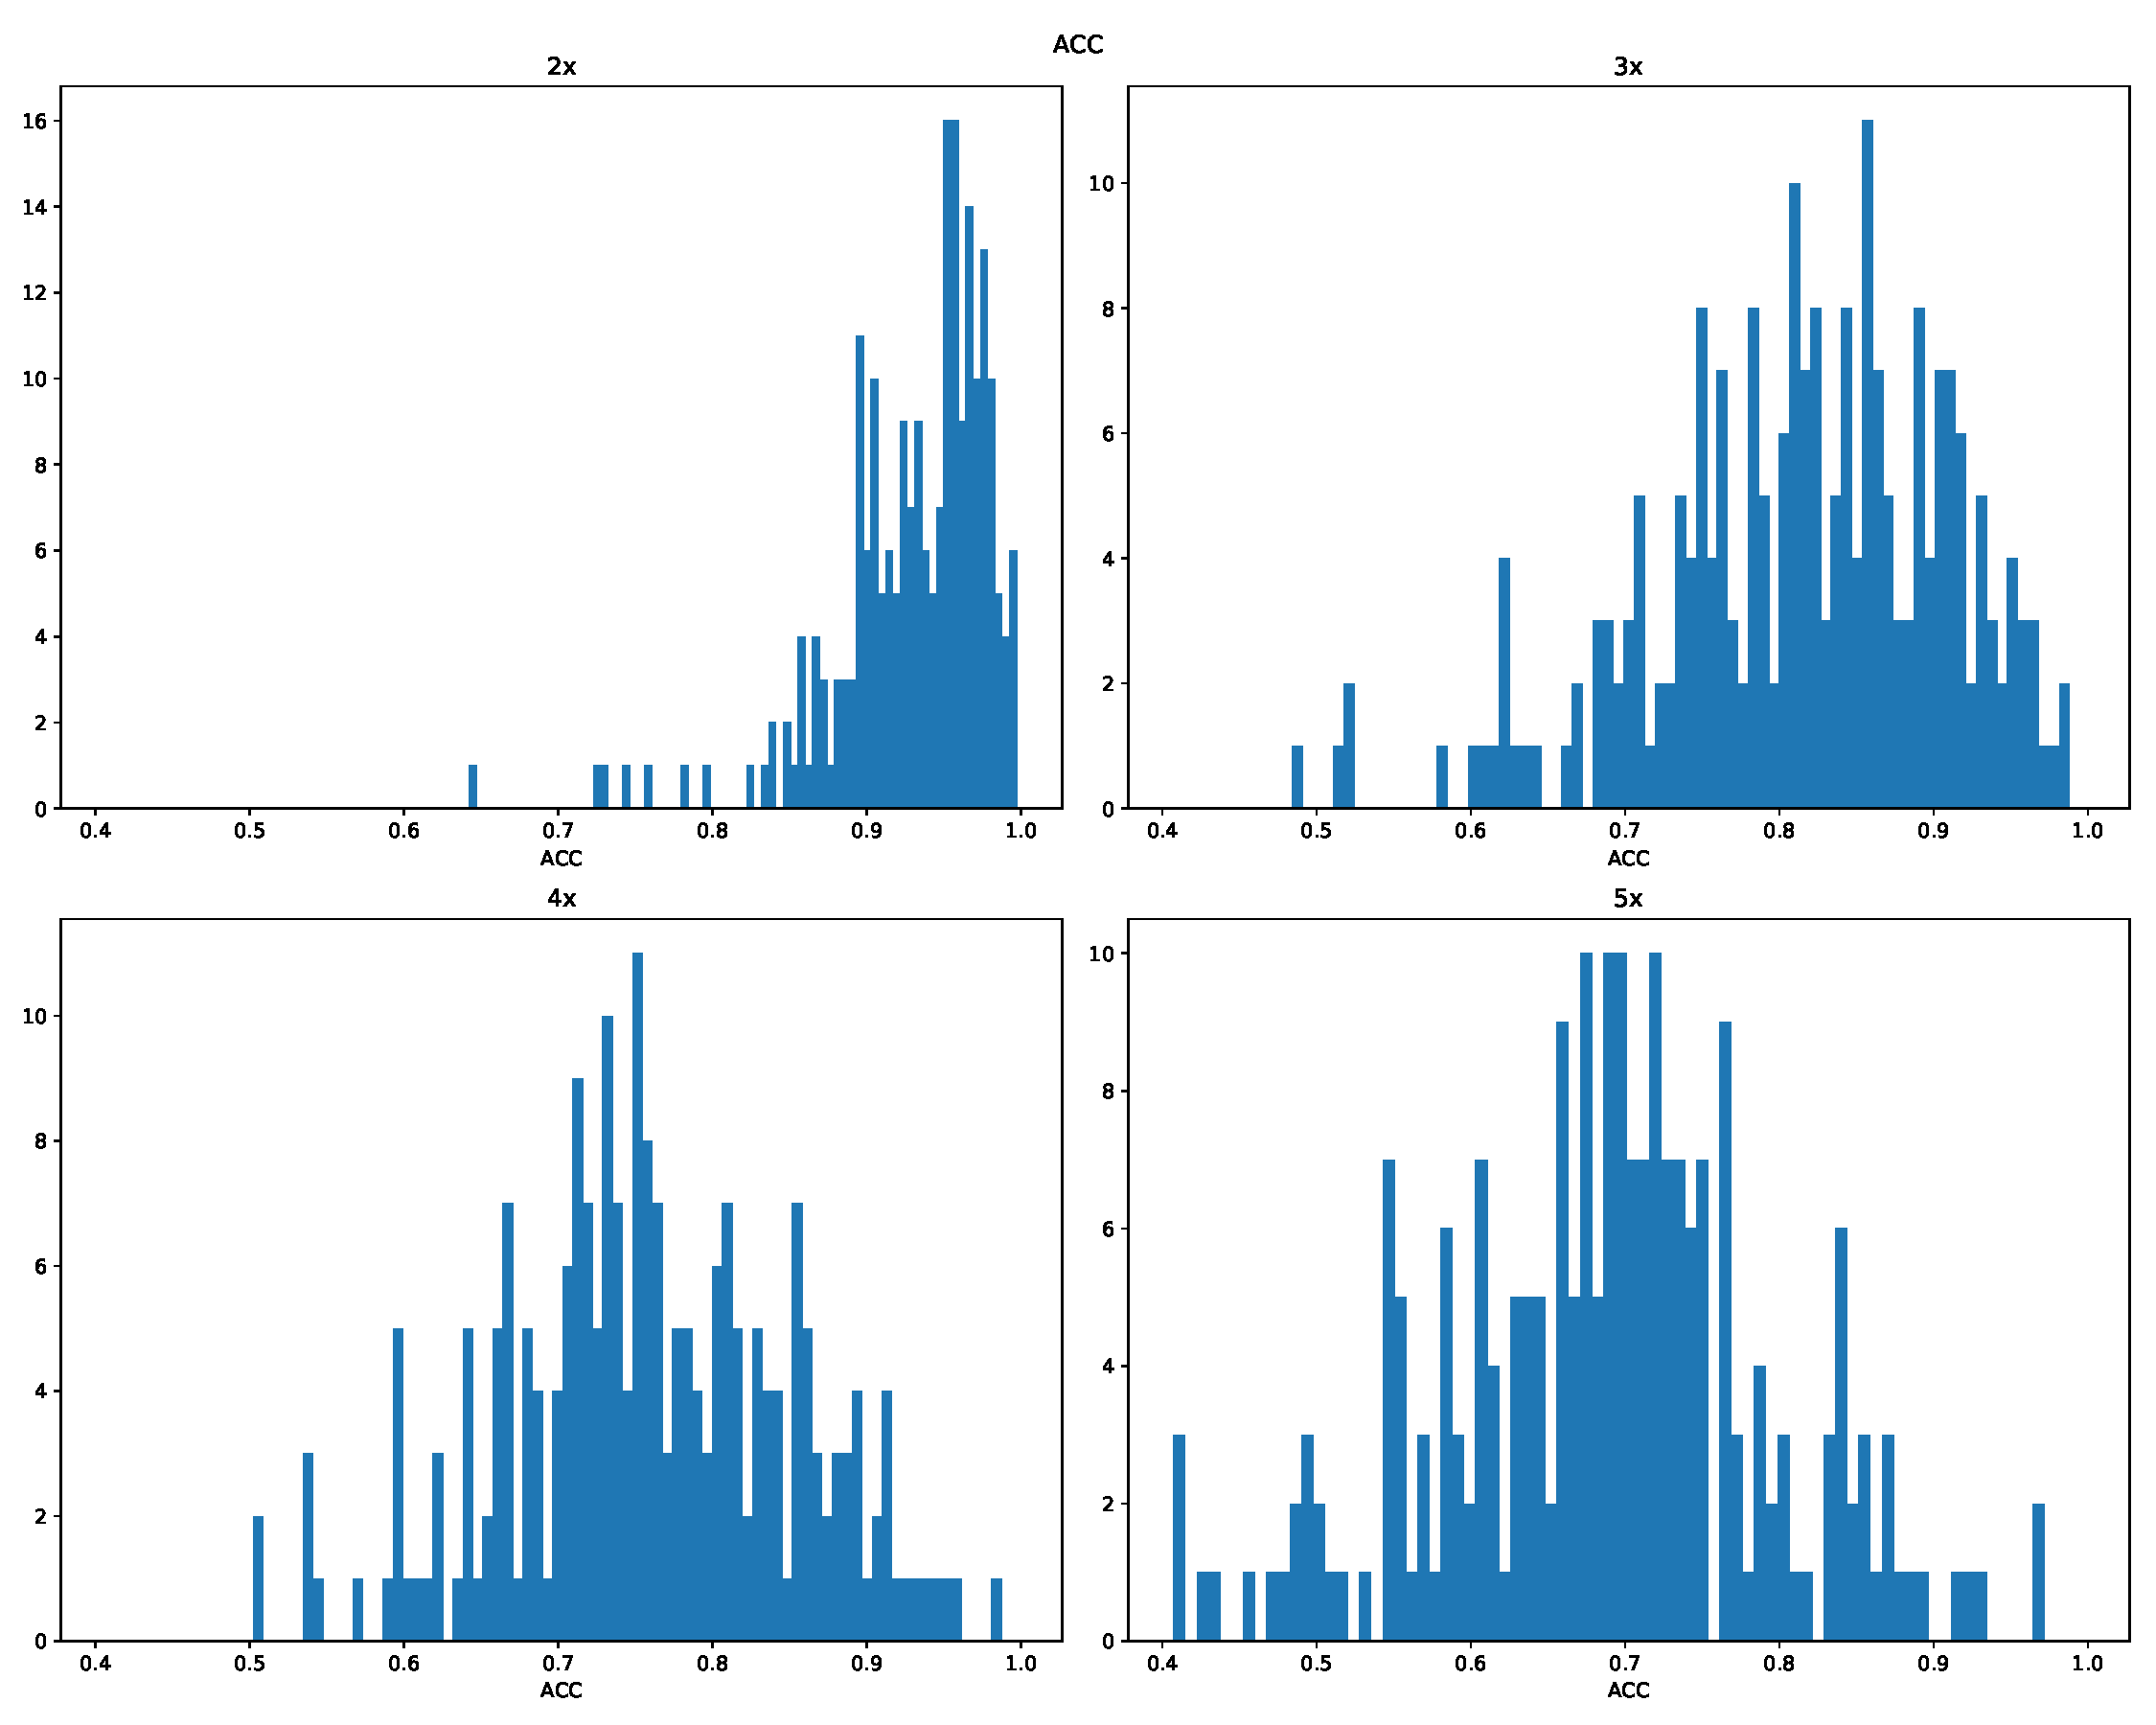
\includegraphics[width=\linewidth]{../plots/ACC}
  \caption{Full ACC distributions}
  \label{fig:acc}
\end{figure}

\begin{figure}[h]
  \centering
  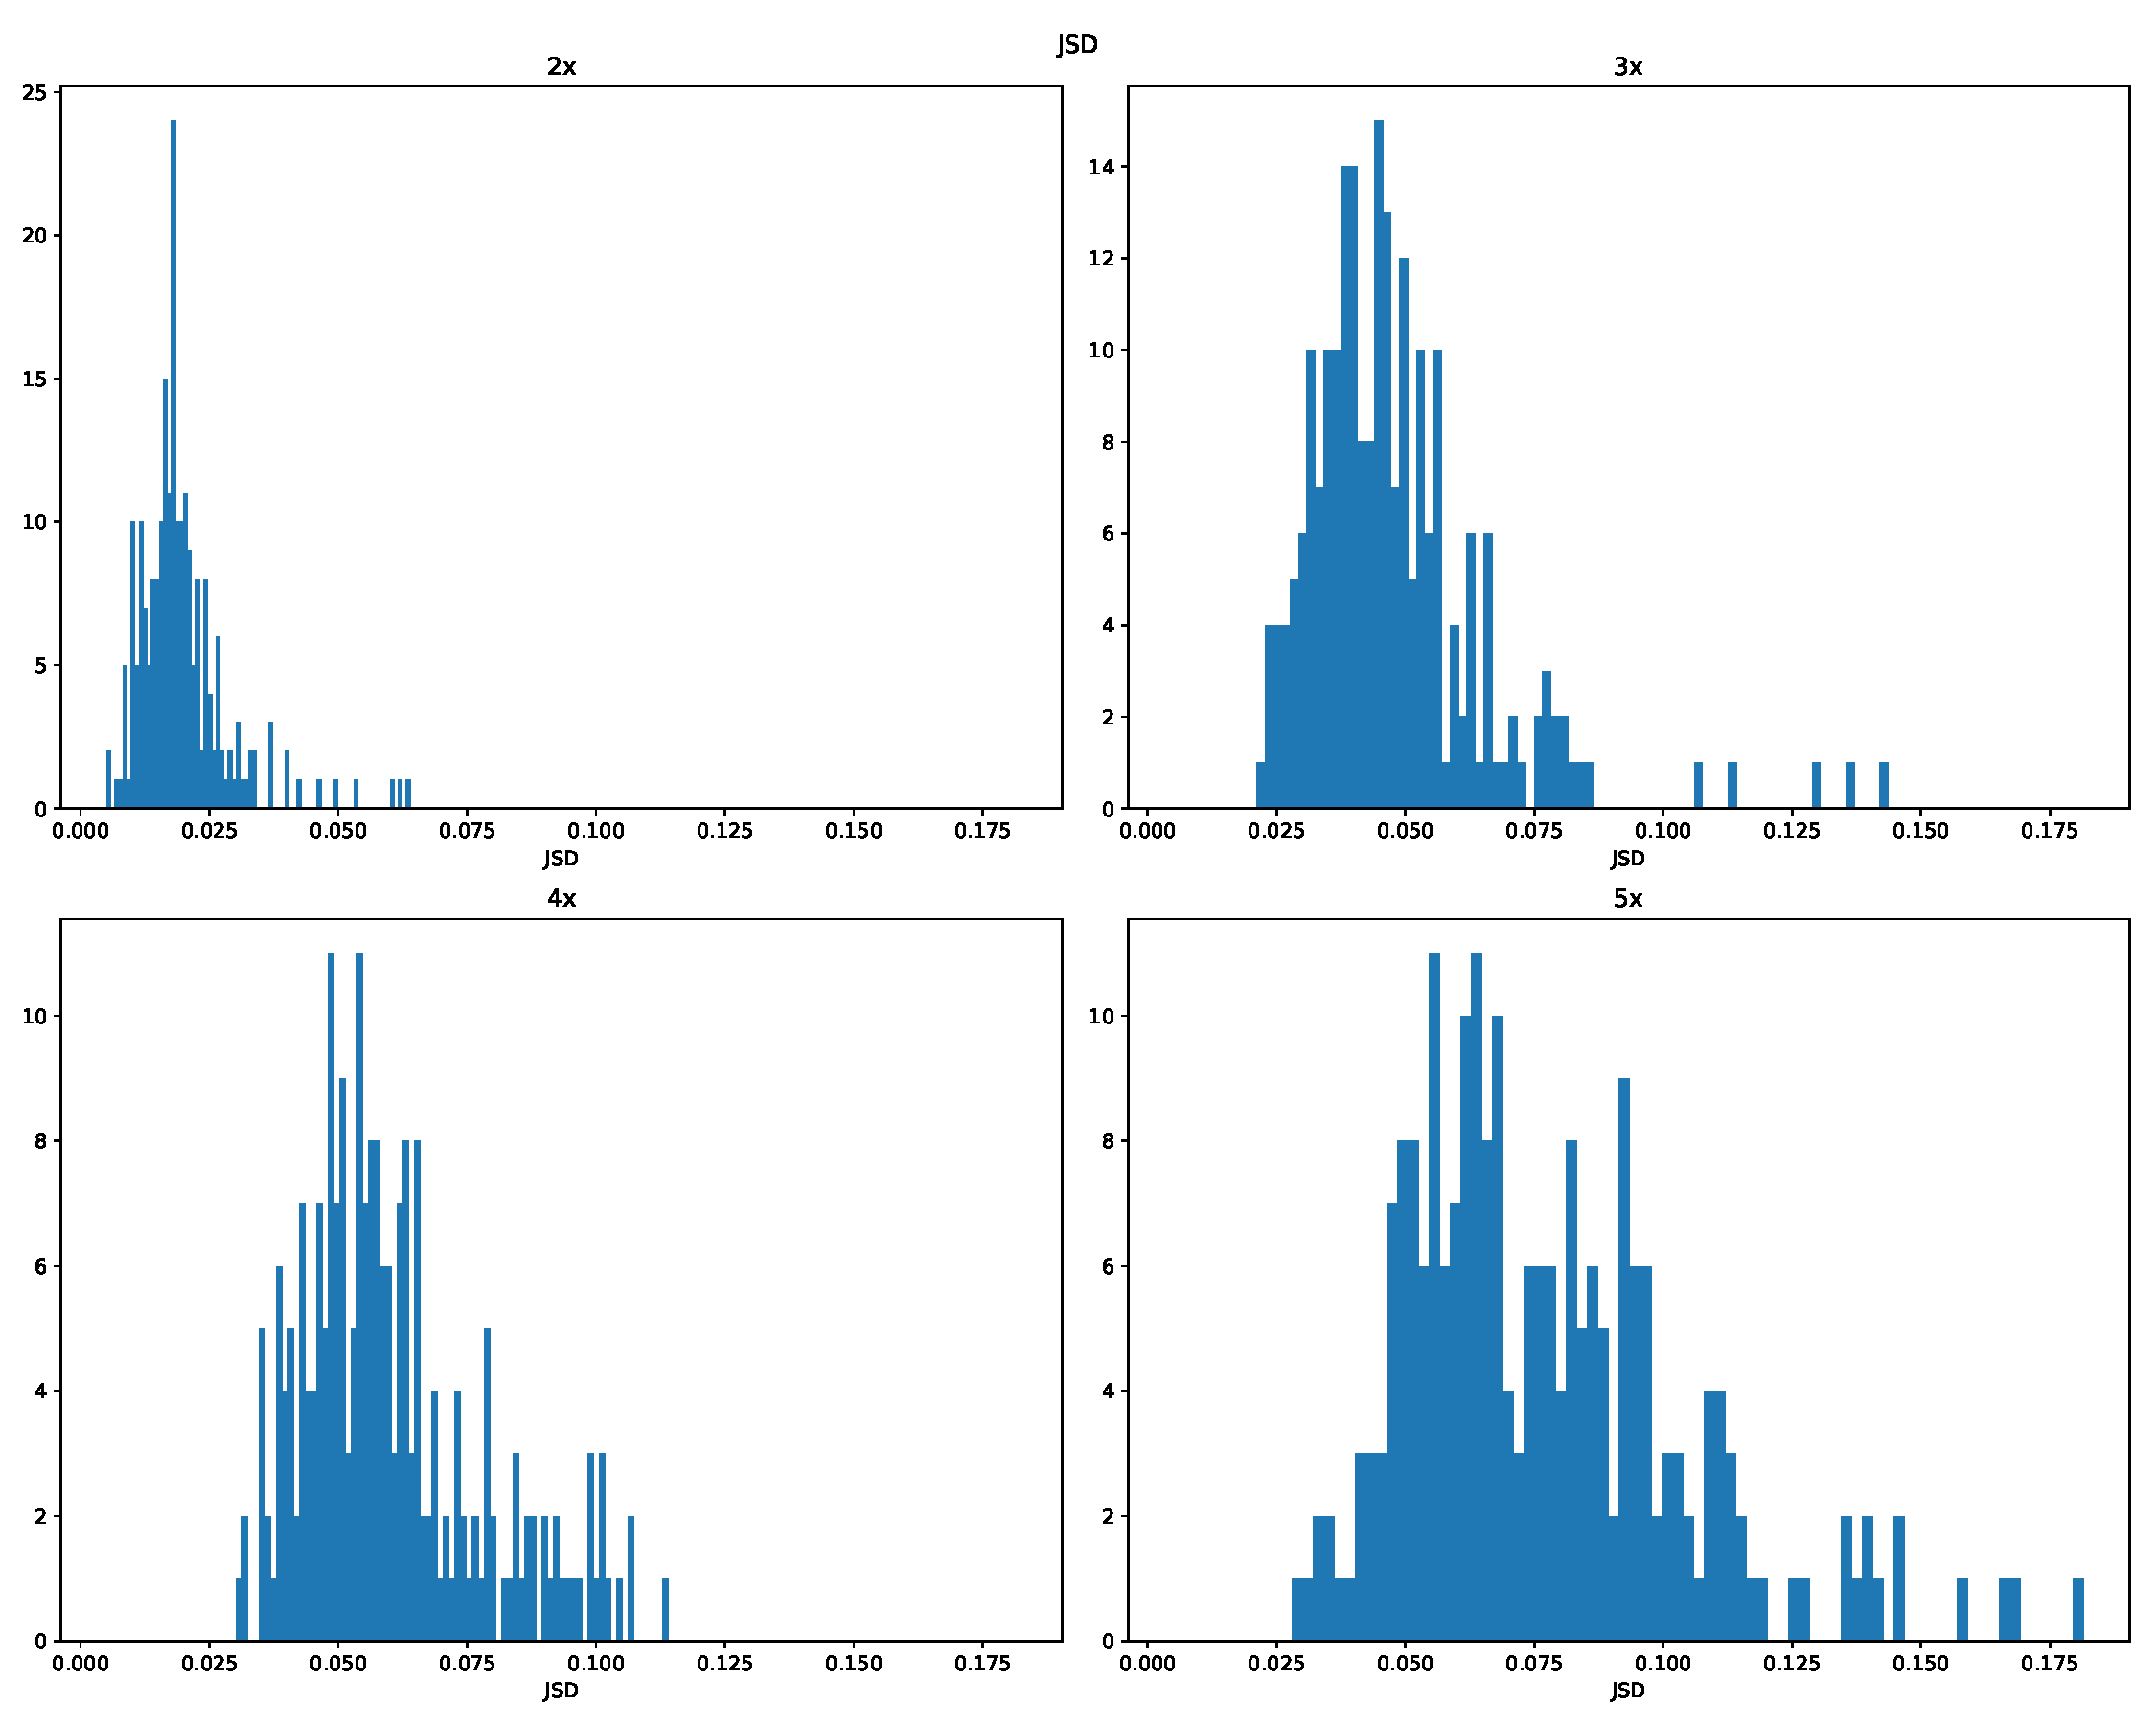
\includegraphics[width=\linewidth]{../plots/JSD}
  \caption{Full JSD distributions}
  \label{fig:jsd}
\end{figure}

\begin{figure}[h]
  \centering
  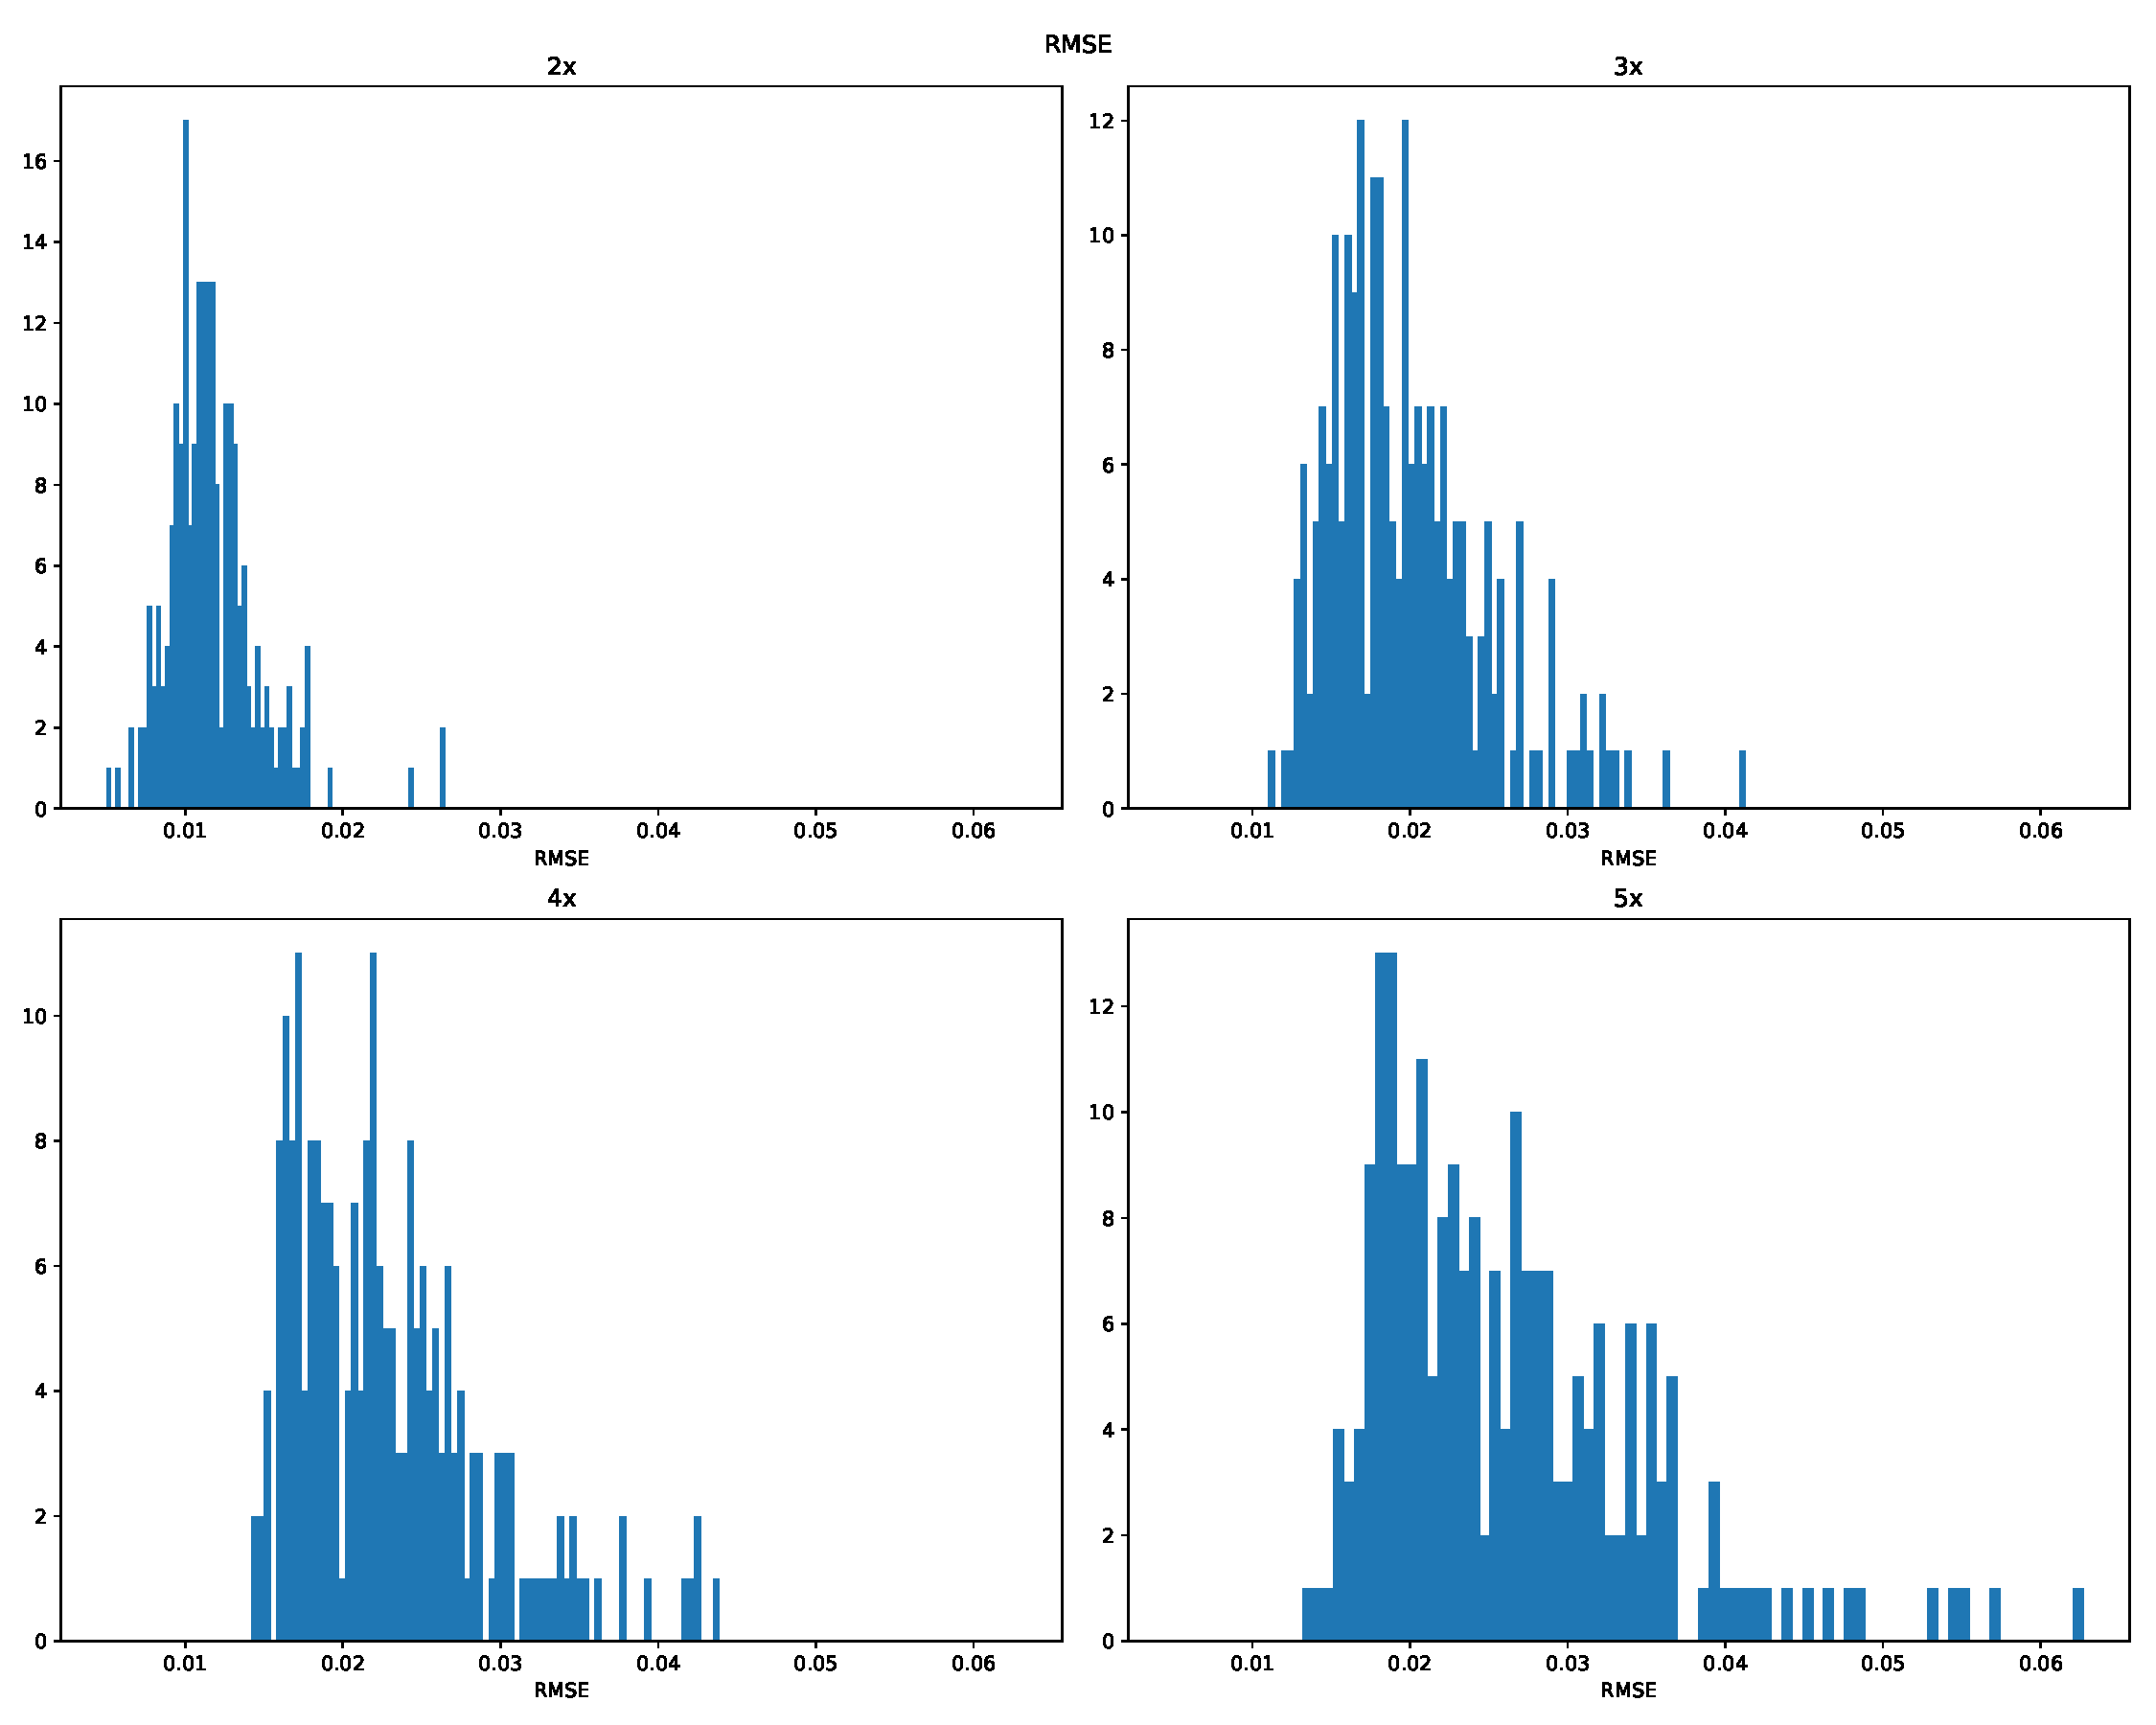
\includegraphics[width=\linewidth]{../plots/RMSE}
  \caption{Full RMSE distributions}
  \label{fig:rmse}
\end{figure}

\begin{figure}[h]
  \centering
  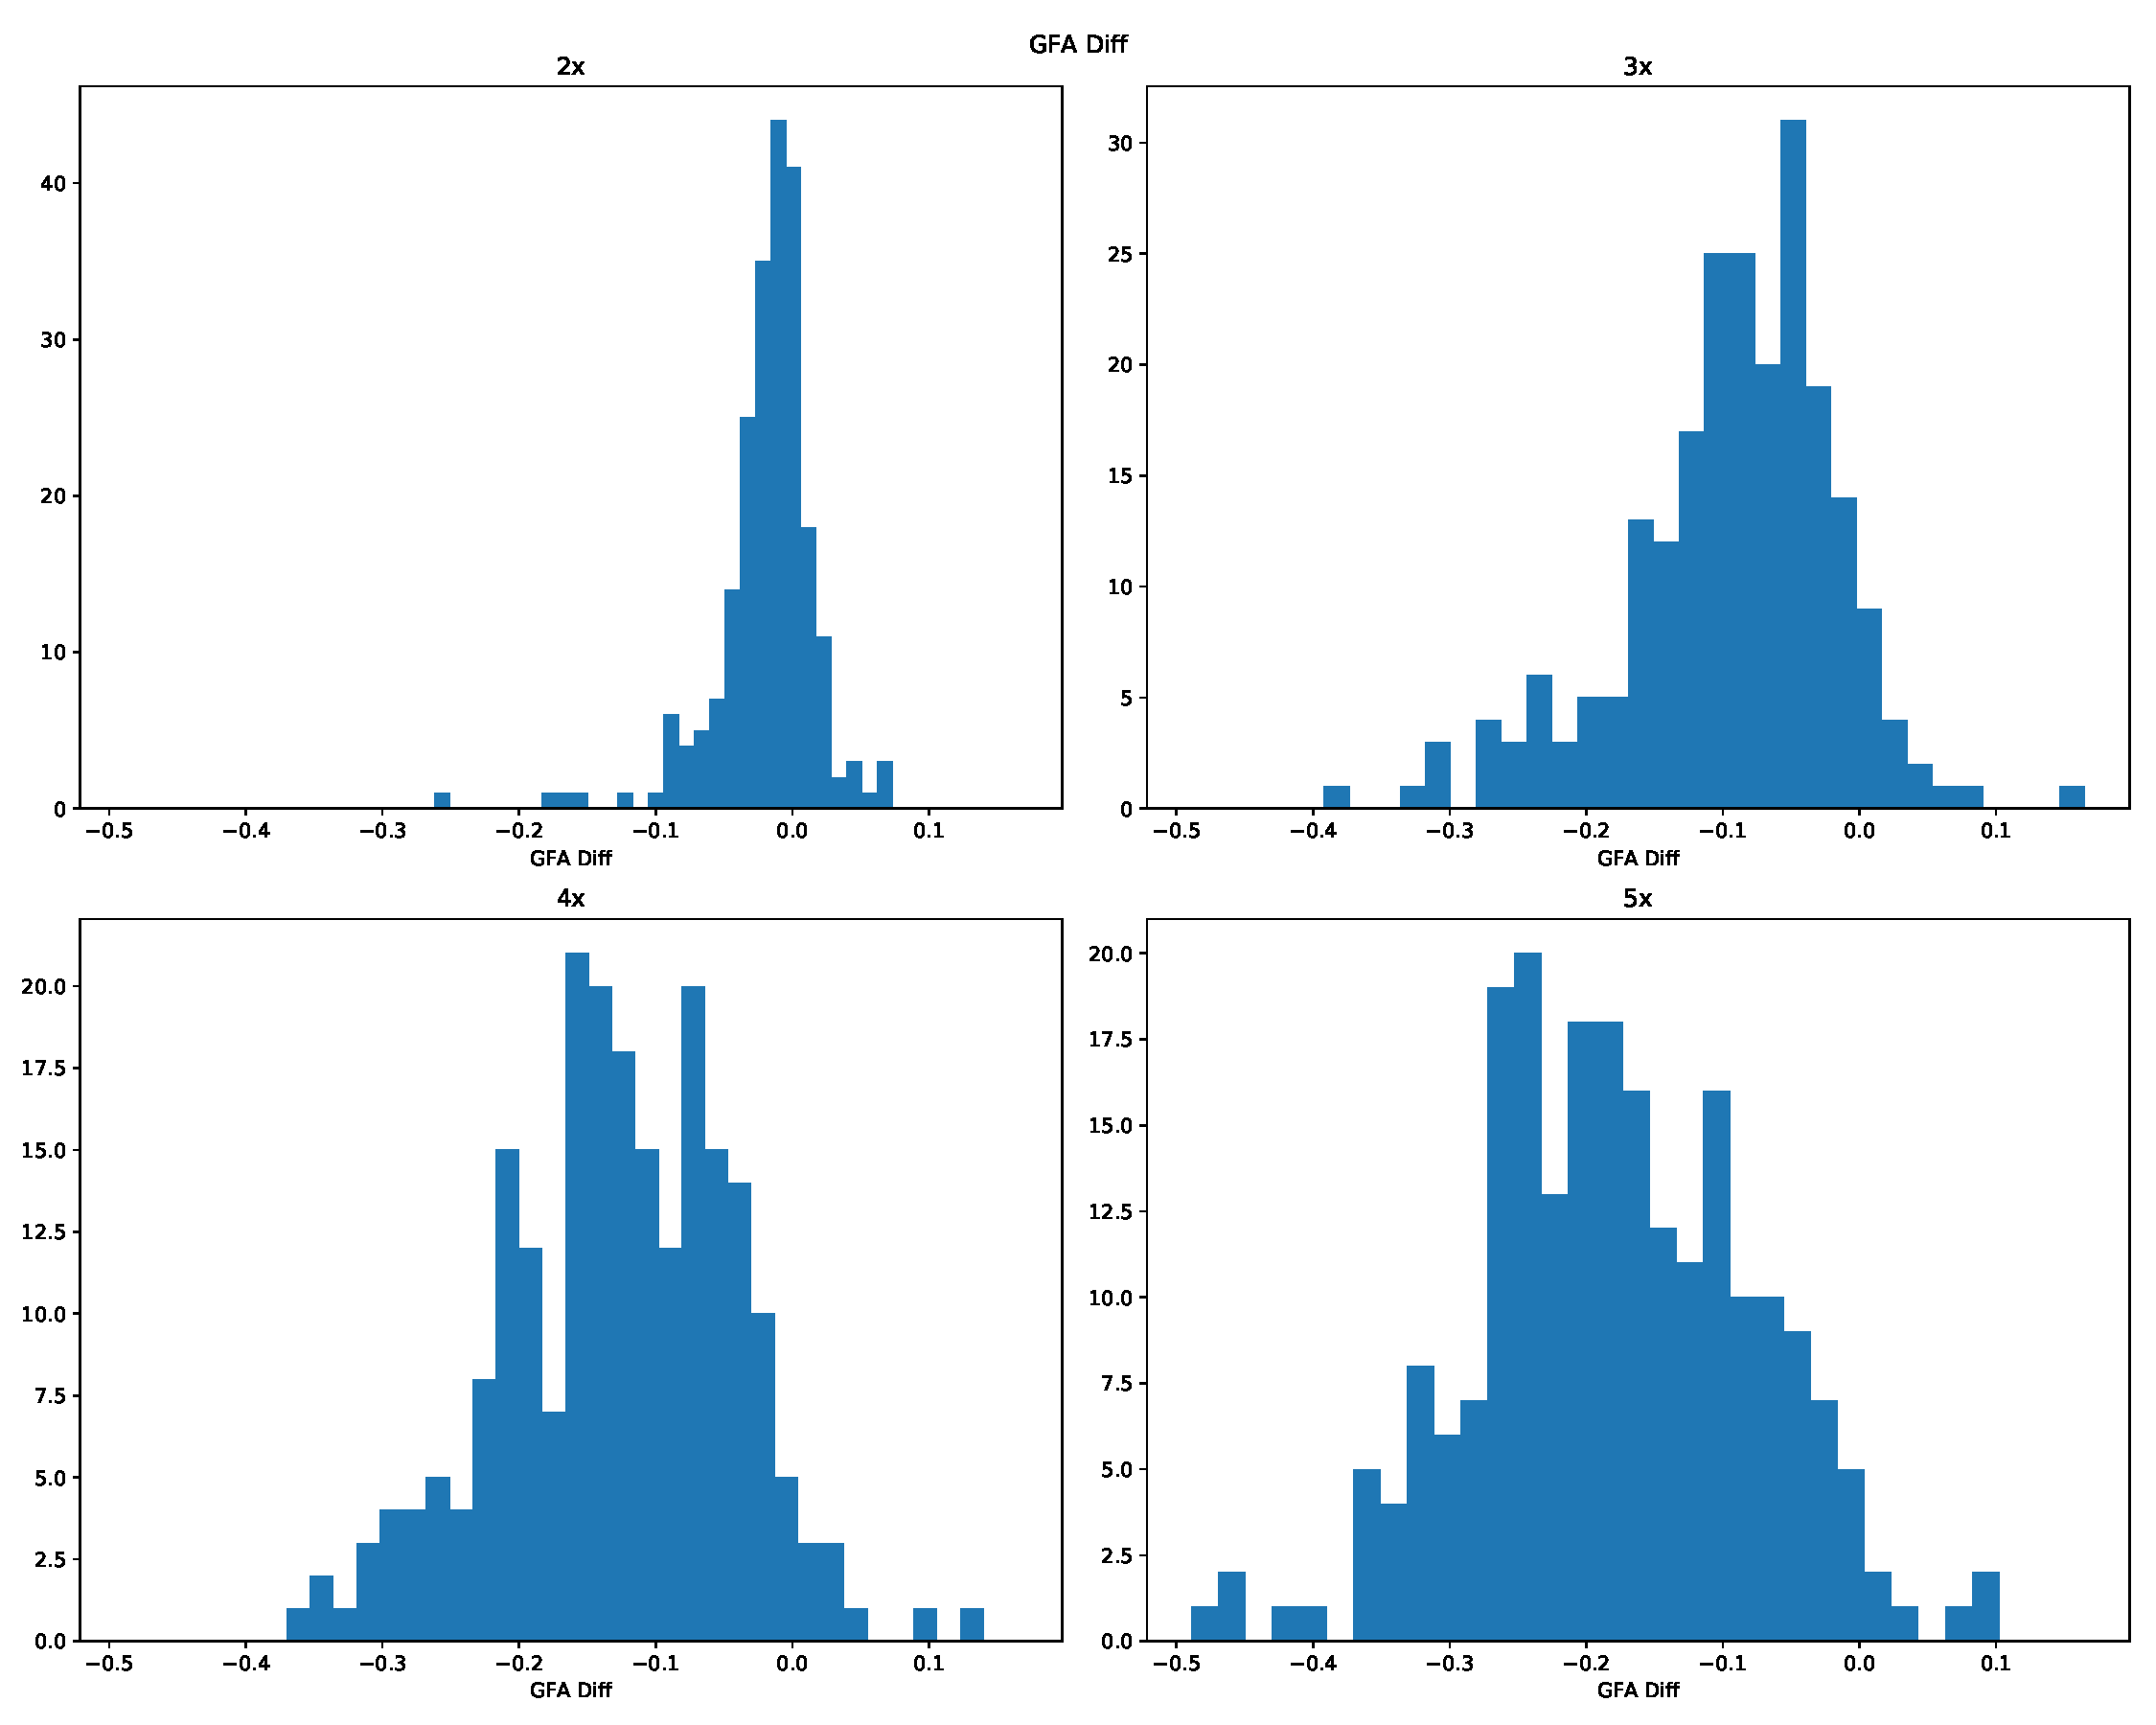
\includegraphics[width=\linewidth]{../plots/GFA_Diff}
  \caption{Full $\Delta$GFA distributions}
  \label{fig:gfa}
\end{figure}

\end{document}
